
\chapter{Impact of current memory management techniques in derived cloud}

  The following set of experiments tries to establish the implications of previously established inferences, as to how these affect 
applications running on a derived cloud environment.
  
  \vspace*{2em}
  \noindent \textbf{Base configuration}
    
  All experiments were configured with 4 containers. Containers contained server workloads (Redis/MongoDB) to which clients had to 
connect. There were two types of containers for each workload i.e Redis and MongoDB. One of each with low priority and other of each with 
higher priority. 

The relative avg. usage of the low : higher priority containers are in the ratio of 1:2 and so are their provisioning. Such provisioning 
makes us \textbf{expect as 1:1 throughput} in terms of application performance between the low and high priority workloads in each case in 
an ideal scenario. The default configurations for the four containers are given on Table:\ref{table_deafult_config}.

    \begin{table}[!htb]
      \begin{center}	   
	\begin{tabular}{ l | p{2cm} | p{2cm} | p{4cm} | p{2cm} }
	  Container & HL (GB) & SL (GB) & Workload Size (records) & Avg. Usage (GB) \\ 
	  \hline
	  \hline
	  Redis-Low & 2 & 0.5 & 500K & 1.3 \\  
	  \hline
	  Mongo-Low & 2 & 0.5 & 500K & 1.3 \\
	  \hline
	  Redis-High & 4 & 1 & 1000K & 2.6 \\  
	  \hline
	  Mongo-High & 4 & 1 & 1000K & 2.6
	\end{tabular}	  
      \end{center}
      \caption{Base configuration for derived cloud experimentation}
      \label{table_deafult_config}	  
    \end{table}

    Containers were created and datasets were loaded off-line to generated the initial memory pressure required. Each container 
had only two clients attached to each of them to avoid CPU bounded contention. The clients were setup on VM-2. All containers were 
over provisioned for all resources other than memory.     
    
    \noindent \textbf{Experimental Flow}
    
    Initially 100s was given to allow the containers to setup and consume desired memory without any external pressure. Once they 
settled, pressure was constantly generated at a rate of x GB every 30s from the host using a balloon driver to constantly reduce the 
memory available to VM-1. Experiments were carried out by varying soft limits, workload size (usage) and external pressure (generated by 
balloon driver). 
    
    \section{Impact analysis}
    
      This section presents the empirical analysis in the derivative cloud environment to see how it impacts real applications.
    
      \subsection{Reclamation when all containers are exceeding}
      
	\begin{figure*}[t!]
	  \centering
	  \begin{subfigure}[t]{0.48\textwidth}
	    \centering
	    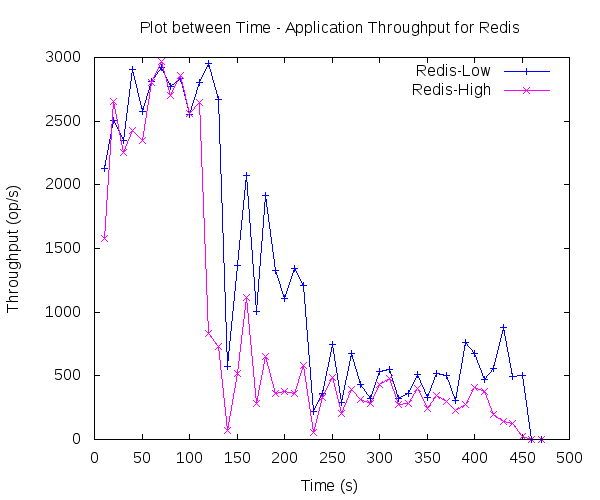
\includegraphics[width=1\textwidth]{images/inference/above_sl_redis.png}
	    \caption{Throughput of Redis containers}
	    \label{plot_inference_above_sl_redis}
	  \end{subfigure}
	  ~ 
	  \begin{subfigure}[t]{0.48\textwidth}
	    \centering
	    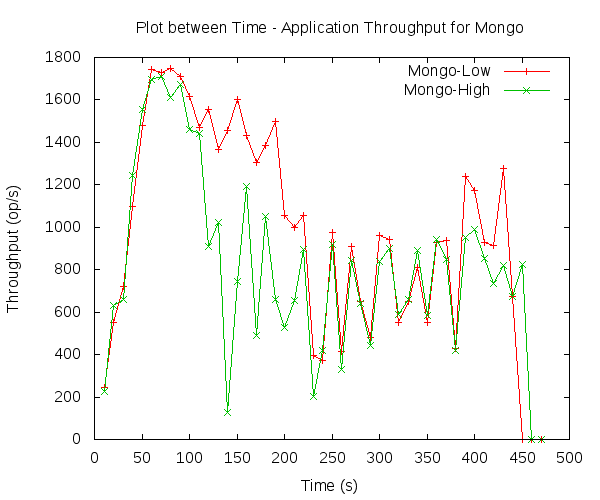
\includegraphics[width=1\textwidth]{images/inference/above_sl_mongo.png}
	    \caption{Throughput of MongoDB containers}
	    \label{plot_inference_above_sl_mongo}
	  \end{subfigure}
	  ~ 
	  \begin{subfigure}[t]{0.48\textwidth}
	    \centering
	    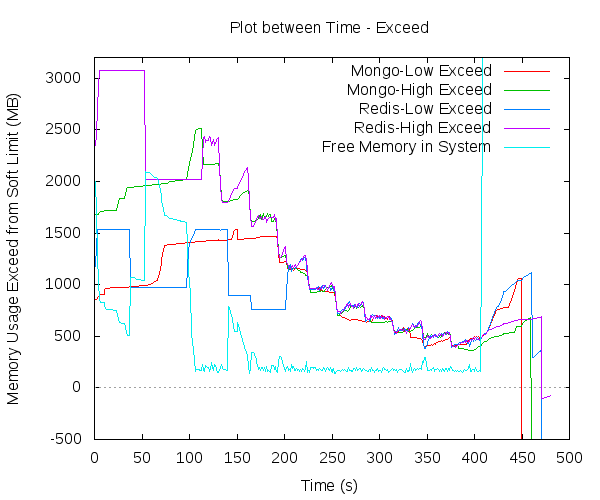
\includegraphics[width=1\textwidth]{images/inference/above_sl.png}
	    \caption{Exceed Plot}
	    \label{plot_inference_above_sl}
	  \end{subfigure}
	  \caption{Plots for analysis while all containers exceeding}
	\end{figure*}
	
	\subsubsection{Question:}
	  \begin{enumerate}	    
	    \item How does reclamation affect applications all containers are exceeding ?
	    \item When containers are exceeding by the different values, in what order and how much of memory reclamation occurs from 
different containers ?
	  \end{enumerate}	
	
	\subsubsection{Procedure:}
	  We begin with containers configured as described in Table:\ref{table_deafult_config}. The balloon driver is inflated inside the 
guest to change memory inside VM in steps of 16-15-14-13-12-11-10.5-10-9.5-9 GB every 30s. 
	
	\subsubsection{Observations:}
	  \begin{enumerate}
	    \item Fig:\ref{plot_inference_above_sl_mongo}, Fig:\ref{plot_inference_above_sl_redis}  shows how application throughput of 
both MongoDB and Redis reach desired throughputs when there is no external pressure in the initial 100s.
	    \item However when pressure kicks in after 100s, the higher priority containers performance degrades drastically. 
	    \item Fig:\ref{plot_inference_above_sl} shows how higher priority containers are penalized more while reclamation which reason 
for the observed decline in application throughput.   
	    \item Fig:\ref{plot_inference_above_sl_mongo} and Fig:\ref{plot_inference_above_sl_redis} shows how each of their containers 
that were better provisioned in memory limits are targeted negatively due to their exceeds.
	  \end{enumerate}
	  
	\subsubsection{Inferences:}
	  \begin{enumerate}
	    \item Exceed based reclamation will negatively impact containers that are provisioned with more memory but are just exceeding 
by greater values.
	    \item Containers with different exceeds equalize and then reclaim alternatively.
	  \end{enumerate}

	  
    \subsection{Reclamation when none of the containers are exceeding}
	
	\begin{figure*}[t!]
	  \centering
	  \begin{subfigure}[t]{0.48\textwidth}
	    \centering
	    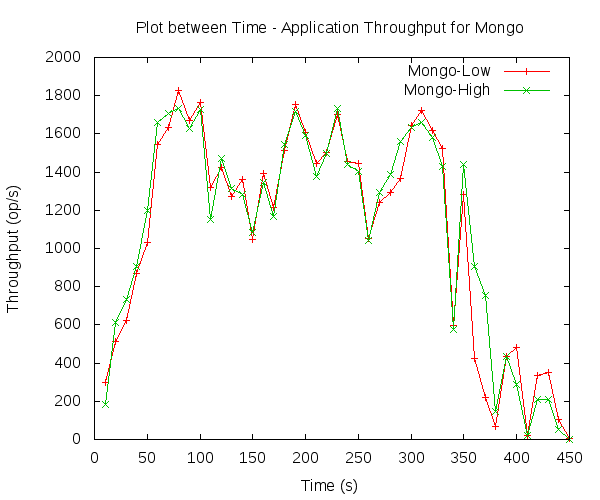
\includegraphics[width=1\textwidth]{images/inference/below_sl_mongo.png}
	    \caption{Throughput of MongoDB containers}
	    \label{plot_inference_below_sl_mongo}
	  \end{subfigure}
	  ~ 
	  \begin{subfigure}[t]{0.48\textwidth}
	    \centering
	    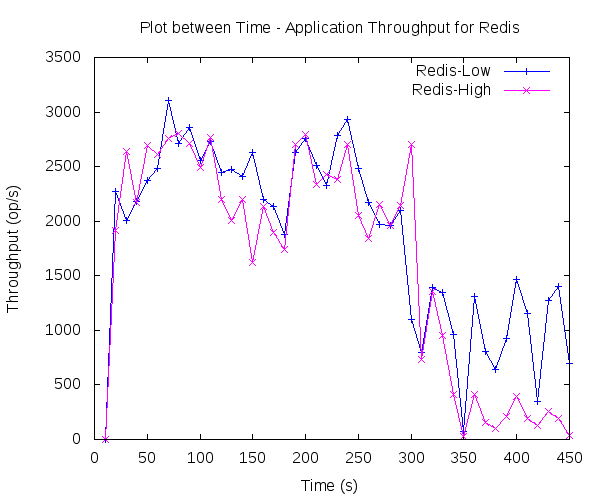
\includegraphics[width=1\textwidth]{images/inference/below_sl_redis.png}
	    \caption{Throughput of Redis containers}
	    \label{plot_inference_below_sl_redis}
	  \end{subfigure}
	  ~ 
	  \begin{subfigure}[t]{0.48\textwidth}
	    \centering
	    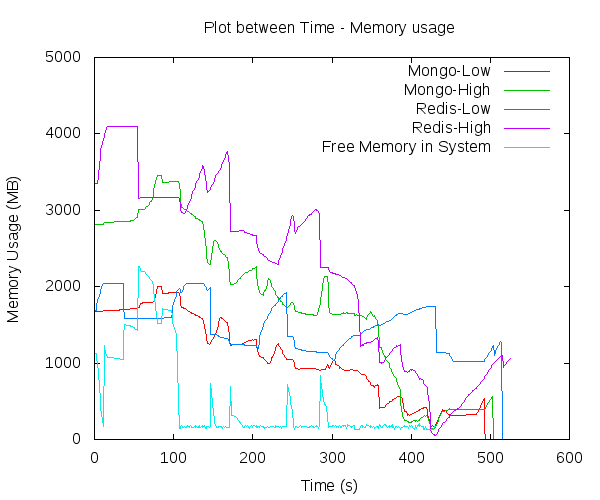
\includegraphics[width=1\textwidth]{images/inference/below_sl.png}
	    \caption{Memory usage plot}
	    \label{plot_inference_below_sl}
	  \end{subfigure}
	  \caption{Plots for analysis when none of the containers are exceeding}
	\end{figure*}
	
	\subsubsection{Question:}
	  \begin{enumerate}	    
	    \item How does reclamation affect applications when none of the containers are exceeding ?
	    \item Are the application performance similar to how it occurs above exceeds ?
	  \end{enumerate}	
	
	\subsubsection{Procedure:}
	  We begin with containers configured as described in Table:\ref{table_deafult_config}. We increase the soft limits of each 
container upto its hard limits to simulate a situation where initial usage of the containers are below soft limits. The balloon driver is 
inflated inside the guest to change memory inside VM in steps of 16-14-12-10-9-8-7-6-5-4-3 GB every 30s. 
	
	\subsubsection{Observations:}
	  \begin{enumerate}
	    \item Fig:\ref{plot_inference_below_sl_mongo}, shows how application throughput of MongoDB almost reaches desired 
throughputs, although their throughputs never stabilize.
	    \item Fig:\ref{plot_inference_below_sl_redis}, shows how application throughput of Redis penalizes the higher priority 
containers due to more pages in its LRU list.
	    \item The unstable throughputs observed in MongoDB and negatively impacted throughputs observed in the case of Redis can be 
accounted to the non-determinism of the GLR which to containers below SL as shown in Fig:\ref{plot_inference_above_sl}. 
	  \end{enumerate}
	  
	\subsubsection{Inferences:}
	  \begin{enumerate}
	    \item GLR based reclamation is non-deterministic which is highly undesirable quality while looking for deterministic 
provisioning.
	  \end{enumerate}
	
    \subsection{Complete reclamation}
	
	\begin{figure*}[t!]
	  \centering
	  \begin{subfigure}[t]{0.48\textwidth}
	    \centering
	    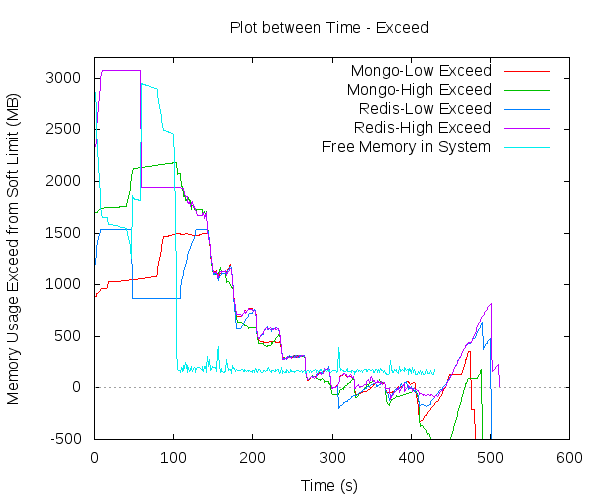
\includegraphics[width=1\textwidth]{images/inference/complete.png}
	    \caption{Exceed plot}
	    \label{plot_inference_complete}
	  \end{subfigure}
	  ~ 
	  \begin{subfigure}[t]{0.48\textwidth}
	    \centering
	    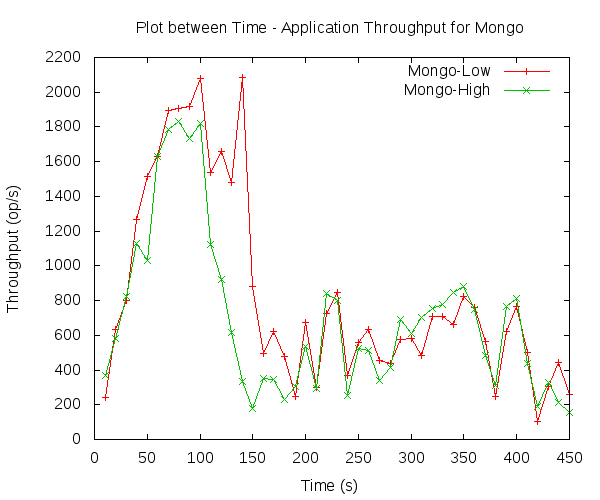
\includegraphics[width=1\textwidth]{images/inference/complete_mongo.png}
	    \caption{Throughput of MongoDB containers}
	    \label{plot_inference_complete_mongo}
	  \end{subfigure}
	  ~ 
	  \begin{subfigure}[t]{0.48\textwidth}
	    \centering
	    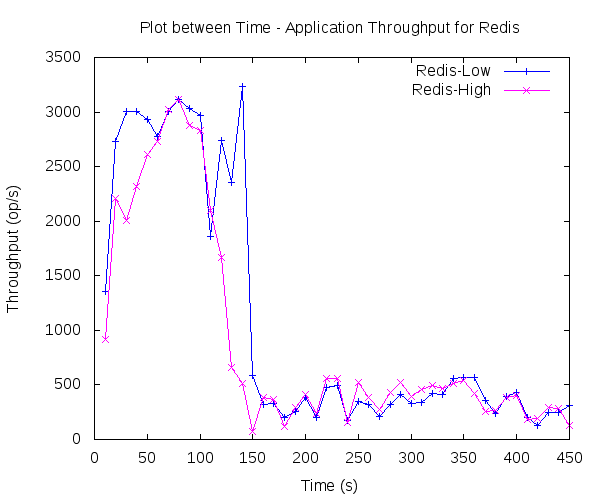
\includegraphics[width=1\textwidth]{images/inference/complete_redis.png}
	    \caption{Throughput of Redis containers}
	    \label{plot_inference_complete_redis}
	  \end{subfigure}
	  \caption{Plots for analysis of complete reclamation starting from exceeding containers to when they aren't}
	\end{figure*}
	
	\subsubsection{Question:}
	  \begin{enumerate}	    
	    \item How does the entire process of reclamation after throughput of containers moving from all containers exceeding to none of 
them exceeding ?
	  \end{enumerate}	
	
	\subsubsection{Procedure:}
	  We begin with containers configured as described in Table:\ref{table_deafult_config}. The balloon driver is inflated inside the 
guest to change memory inside VM in steps of 16-14-12-10-9-8-7-6-5-4-3 GB every 30s. 
	
	\subsubsection{Observations:}
	  \begin{enumerate}
	    \item Fig:\ref{plot_inference_complete_mongo}, Fig:\ref{plot_inference_below_sl_redis} shows how application throughput of 
MongoDB and Redis is impacted negatively using the existing knobs when provisioning for deterministic allocation as observed in between 
t=100 and t=200.
	    \item When reclamation goes agnostic of existing knobs (after t=200), it appears to have more desired throughputs but this 
maybe accounted for the nature of the current workloads that actively consume memory. 
	    \item  In case of a workload that uses memory after certain intervals, this situation may achieve undesired throughputs even 
below soft limits. This needs further experimentation.
	    \item As observed here container soft limits are violated when the system is under immense pressure or the container soft 
limits are over provisioned. However, the system tries its best efforts to maintain soft limits.  
	  \end{enumerate}
	  
	\subsubsection{Inferences:}
	  \begin{enumerate}
	    \item The container aware reclamation above soft limits impact negatively in when trying to achieve deterministic provisioning 
with QOS guarantees.
	    \item There is a lot of non determinism in reclamations below soft limits in the current policy.
	    \item Soft limits are not guarantees, but are mere best effort approach.
	  \end{enumerate}

  \section{Key sights and drawbacks of existing system}
    \begin{enumerate}
      \item Reclamation above SL is based on exceed values of each container, may impact negatively while we try to provision containers 
based on QOS guarantees.
      \item Reclamation below SL falls back to host LRU based reclamation without taking into container provisioning and this leads to a 
lot of non-determinism.
      \item Soft Limit is not a definite guarantee, it is mere best effort approach.
    \end{enumerate}